
\documentclass[tikz,border=12pt]{standalone}
\usepackage{tikz}
\usepackage{amsmath}
\usetikzlibrary{arrows.meta,calc,positioning,shapes.geometric}

\begin{document}

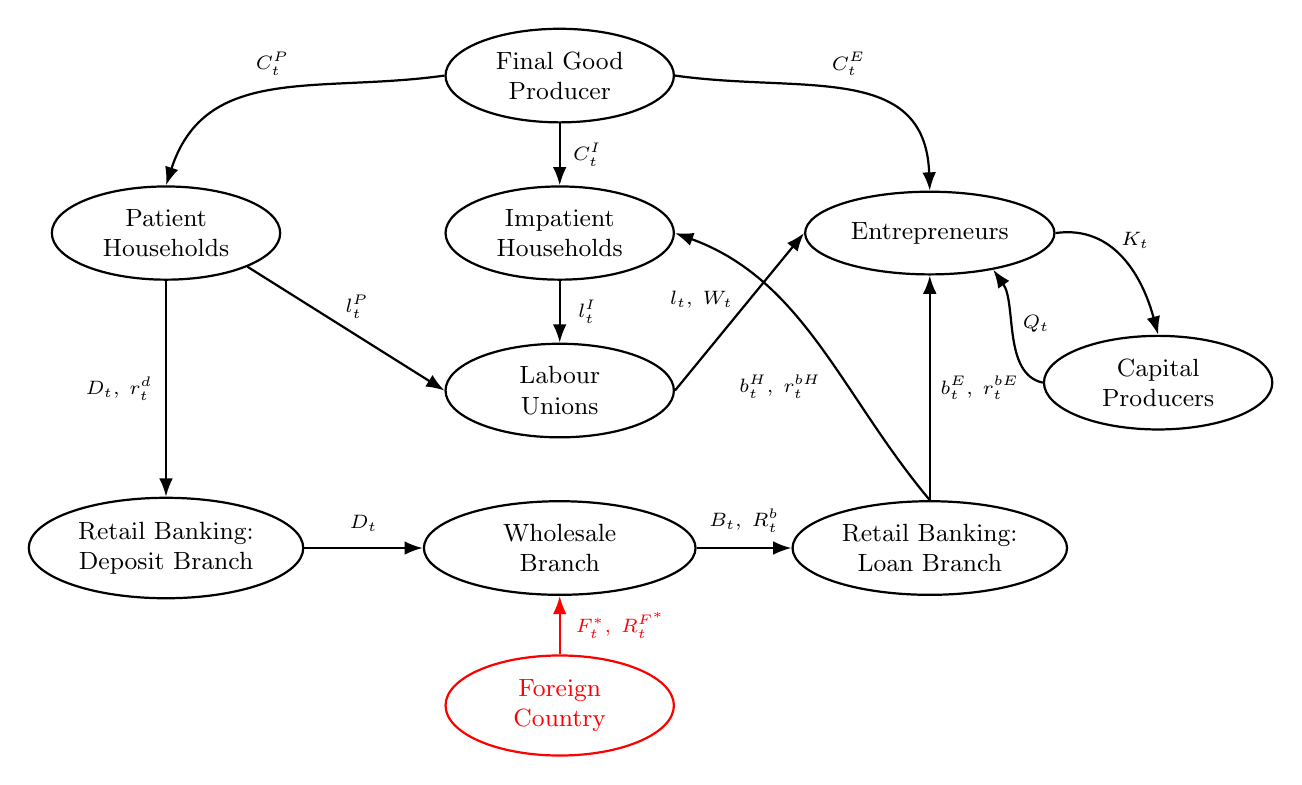
\begin{tikzpicture}[
    >=Latex,
    thick,
    every node/.style={font=\small},
    agent/.style={
        draw,
        ellipse,
        minimum width=2.9cm,
        minimum height=1.05cm,
        align=center
    },
    bank/.style={
        draw,
        ellipse,
        minimum width=3.45cm,
        minimum height=1.12cm,
        align=center
    },
    flow/.style={->, thick},
    extflow/.style={->, thick, red},
    lab/.style={
        font=\scriptsize,
        fill=white,
        inner sep=1.0pt,
        text=black
    },
    extlab/.style={
        font=\scriptsize,
        fill=white,
        inner sep=1.0pt,
        text=red
    }
]

%------------------------------------------------
% Nodes
%------------------------------------------------
\node[agent] (fgp)  at (0.0,4.45)   {Final Good\\Producer};

\node[agent] (ph)   at (-5.0,2.45)  {Patient\\Households};
\node[agent] (ih)   at (0.0,2.45)   {Impatient\\Households};
\node[agent] (e)    at (4.7,2.45)   {Entrepreneurs};

\node[agent] (lu)   at (0.0,0.45)   {Labour\\Unions};
\node[agent] (cp)   at (7.6,0.55)   {Capital\\Producers};

\node[bank]  (rbdb) at (-5.0,-1.55) {Retail Banking:\\Deposit Branch};
\node[bank]  (wb)   at (0.0,-1.55)  {Wholesale\\Branch};
\node[bank]  (rblb) at (4.7,-1.55)  {Retail Banking:\\Loan Branch};

\node[agent, draw=red, text=red] (fc) at (0.0,-3.55) {Foreign\\Country};

%------------------------------------------------
% Arrows and standard labels
%------------------------------------------------

\draw[flow] (fgp.west) to[out=188,in=72,looseness=1.10]
    node[pos=0.50, yshift=10pt, lab] {$C_t^P$}
    (ph.north);

\draw[flow] (fgp.south) --
    node[pos=0.50, xshift=10pt, lab] {$C_t^I$}
    (ih.north);

\draw[flow] (fgp.east) to[out=-8,in=92,looseness=1.18]
    node[pos=0.50, yshift=10pt, lab] {$C_t^E$}
    (e.north);

\draw[flow] (ph.south) --
    node[pos=0.50, xshift=-17pt, lab] {$D_t,\; r_t^d$}
    (rbdb.north);

\draw[flow] (ph.south east) --
    node[pos=0.50, xshift=4pt, yshift=8pt, lab] {$l_t^P$}
    (lu.west);

\draw[flow] (ih.south) --
    node[pos=0.50, xshift=10pt, lab] {$l_t^I$}
    (lu.north);

\draw[flow] (lu.east) -- (e.west);

\draw[flow] (rbdb.east) --
    node[pos=0.50, yshift=9pt, lab] {$D_t$}
    (wb.west);

\draw[flow] (wb.east) --
    node[pos=0.50, yshift=10pt, lab] {$B_t,\; R_t^b$}
    (rblb.west);

\draw[extflow] (fc.north) --
    node[pos=0.50, xshift=22pt, extlab] {$F_t^{*},\; R_t^{F^{*}}$}
    (wb.south);

\draw[flow] (rblb.north) --
    node[pos=0.50, xshift=18pt, lab] {$b_t^E,\; r_t^{bE}$}
    (e.south);

\draw[flow] (rblb.north) to[out=130,in=-20,looseness=0.95] (ih.east);

% K_t now placed directly on the E -> CP path, centred by path length
% and moved to the upper side with a uniform offset.
\draw[flow] (e.east) to[out=8,in=105,looseness=1.05]
    node[pos=0.57, xshift=2pt, yshift=10pt, lab] {$K_t$}
    (cp.north);

\draw[flow] (cp.west) to[out=168,in=-55,looseness=0.85] (e.330);

%------------------------------------------------
% Manual labels for crowded arrows only
%------------------------------------------------

\node[lab] at (1.8,1.6) {$l_t,\; W_t$};
\node[lab] at (2.8,0.5) {$b_t^H,\; r_t^{bH}$};
\node[lab] at (6.05,1.3) {$Q_t$};

\end{tikzpicture}

\end{document}
